\documentclass[12pt, onecolumn]{article}

\usepackage[utf8]{inputenc}
\usepackage[brazil]{babel}
\usepackage[top=2cm, bottom=2cm, right=2cm, left=2cm]{geometry}


\usepackage{graphicx}
\usepackage{natbib}

	\title{Circuitos Digitais}
	\author{Thiago Figueiredo Marcos}
	\date{\today}

\begin{document}
	
	\maketitle

	\section{\centering Introdução}
	
	Um computador digital pode ser descrito como aquilo que computa, ou aquilo 
	que processa informação digital. A informação que é processada por 
	um circuito digital é aquela que é \textbf{quantizada} ou 
	\textbf{discretada} \citep{art1}. \\
	\newline
	No mundo comum, as informações são analógicas, ou seja, a onda que 
	representa aquela informação possui uma gama de valores diferenciados. 
	Já os sinais digitais podem ser representados apenas por dois valores, 
	ou seja, uma lógica binária \citep{bk1}. \\ 
	\newline
	Os circuitos digitais são construidos por componentes eletrônicos e 
	tem como entradas e saidas sinais digitais. Para usarmos informações 
	do mundo analógico é preciso discretar essas informações, afím de 
	convertelas à binária e geralmente é usado uma medida em Volts para 
	determinar se uma informação é ligada ou desligada. 
	Após convertida a informação e processada no circuito digital é 
	preciso converter o sinal de saída do circuito que é digital, 
	em analógico novamente\citep{art2}.

	\section{\centering Conversão Analógico - Digital (Discretação)}
	
	Sinais discretos são frequências descontinuas no tempo, ou seja, 
	definida apenas para determinados instantes. Representa aproximadamente 
	o mundo real, entretanto, podem ser utilizadas várias técnicas para 
	melhorar a representação, como as de processamento de sinais digitais.\\
	\newline
	Aqui também vale ressaltar que o processo de discretação de alguma 
	informação está consequentemente ligada a perca de determinadas 
	informações.
		
	\subsection{\centering Principais propiedades da discretação}	
	\begin{enumerate}
		\item\textbf{Amostragem}: Discretação do sinal analógico no tempo.
		\item\textbf{Quantização}: Discretação da amplitude 
			do sinal amsotrado em niveis.
		\item\textbf{Codificação}: Atribuição de códigos, onde geralmente 
				são binários às	amplitudes do sinal quantizado.
	\end{enumerate}

	\section{\centering Conversão Digital - Analógico (Linearização)}
	
	Se refere a o processo que transforma um sinal modelado por eventos 
	discretos em um sinal contínuo, ou seja, o processo de integração 
	de vários sinais discretos para simular um evento contínuo.

	\section{\centering Processamento}

	O processamento de informação se refere a diversas operaçõs 
	realizadas por um circuito digital para transformar a entrada 
	de dados em uma saida significativa de interesse.\\
	\newline
	Isso pode ser: calculos, manipular dados como agregação, 
	separação e classificação ou ainda filragem, entre outros. 
	Além disso, no circuito digital é simplificado o 
	armazenamento de informações bem como possui uma menor probabilidade 
	de interferências.
	
	\section{\centering Sistemas de numeração}

	Número nos remete a ideia de quantidade, já o numeral é a 
	representação desta ideia, na prática, nos referimos a palavra 
	número para qualquer tipo de representação numeral. \\
	\newline
	\textbf{Exemplo}: A quantidade \texttt{Quarenta e dois} é representada pelo
	numeral 42.\\
	\newline
	Sem o conhecimento da organização posicional dos números, como podemos
	representar todos eles? Poderiamos pensar em um simbolo para cada número,
	porém, existe uma infinidade de quantidades.\\
	\newline
	Há cerca de 3.000 anos atrás os \texttt{Egípcios} desenvolveram um sistema
	de numeração em base 10, na qual utilizamos até hoje. 
	Os números representados por hieróglifos eram mais usados em 
	monumentos e templos, pintados ou talhados em pedra. Há sete símbolos, 
	representando os números 1, 10, 100, 1000, 10 000, 100 000 e 
	1 000 000 \citep{art3}. \\
	\newline
	Algarismos é um conjunto finito de símbolos numéricos que usamos para
	representar quantidades reais. Todo e qualquer número pode ser representado
	por uma combinação de algarismos, os mais conhecidos são os indo-arábicos:
	0, 1, 2, 3, 4, 5, 6, 7, 8, 9. \\
	\newline
	Sistema de numeração é a forma de atribuir uma representação única para 
	cada número. O sistema de numeração posicional atribui valor 
	ao algarismo conforme a sua posição, mais a esquerda ou mais a direita.
	\newline
	No sistema decimal de numeração posicional possuimos 10 algarismos, 0 .. 9,
	cada um deles representa seu valor absoluto, ou seja, o valor 0 
	representa o nada, o valor 1 representa uma única unidade 
	e assim por diante. Dependendo da posição que o valor estiver, 
	seu valor absoluto pode variar, por exemplo: Imagine um número com 
	4 casas decimais, - - - -, o número que estiver na 'casa' mais a esquerda 
	não representara seu valor absoluto e sim o seu valor
	absoluto multiplicado por um milhão. \\
	\newline
	\textbf{Exemplo}: 4237 = 4*1000 + 2*100 + 3*10 + 7*1, observe o seguinte:\\
	\newline
	4*1000 	= 4.000\\
	2*100 	= 200\\
	3*10	= 30\\
	7*1	= 7\\
	\newline
	A soma de todos os valores resulta no valor original 4.237.\\
	\newline
	Agora podemos sistematizar isso matematicamente, sabemos que um número
	inteiro A no sistema decimal é presentado por N digitos assim:\\
	\begin{center}
		$A_{n-1} A_{n-2} ... A_{n2} A_{n1} A_{n0}$
	\end{center}
	Cada $a_{i}$ é um algarismo decimal.
	\begin{center}
		$a_{n-1}*10^{n-1} + a_{n-2}*10^{n-2}
		+ ... + 
		a_{2}*100 + a_{1} * 10 + a_{0} * 1$
	\end{center}

	ou seja,

	\begin{center}
		$\sum_{i = 0}^{n - 1} a_{i} * 10^{i}$
	\end{center}

	Usando a mesma lógica, podemos representar os números racionais no sistema
	decimal
	
	\begin{center}
		$\sum_{i = 0}^{n - 1} a_{i} * 10^{i} + 
		\sum_{i = 1}^{\infty} a_{-i} * 10^{-i}$
	\end{center}

	\section{\centering Truncamento}

	Vemos que à medida que caminhamos mais a direita depois da virgula, o
	valor relativo a cada algarismo se torna cada vez menor, podemos
	fazer uma representação aproximada do número gerado, limitando 
	o número de algarismos após a vírgula por uma constante \texttt{M}.\\
	\newline
	Essa aproximação chama-se truncamento. Com o truncamento há também
	um erro de aproximaçaõ que pode ser obtido com a diferença do número original
	com o número truncado. \\
	\newline
	Ao truncarmos um número com uma constante \texttt{M} para qualquer 
	número real com n algarismos à esquerda da virgula, 
	e \texttt{M} algarismos à direita, assim: 

	\begin{center}
		$a_{n-1} a_{n-2} ... a_{1} a_{0}, a_{-1} a_{-2} ... a_{M}$
	\end{center}

	então temos que o erro de aproximação de qualquer número N será:

	\begin{center}
		$\texttt{err} < 10^{-M}$
	\end{center}
	
	ou seja, aumentar \texttt{M} implica em diminuir o erro.
	
	\section{\centering Bases não decimais}

	A quantidade de algarismos usados em um sistema de numeração posicional é
	chama de base, por exemplo: O sistema decimal tem 10, 
	o sistema binário tem 2 e assim por diante. \\
	\newline
	Acima fizemos uma representação matemática dos números posicionais 
	racionais, a questão é que, em um sistema posicional em uma determinada
	base \textbf{d}, pode ser representada da seguinte forma: 

	\begin{center}
		$\sum_{i=0}^{n-1} a_{i} * d^{i} + 
		\sum_{i=1}^{\infty} a_{-i} * d^{-i}$
	\end{center}

	Para indicar a base em que um número esta representado é comum a 
	seguinte notação:

	\begin{center}
		$(a_{n-1} a_{n-2} ... a_{1} a_{0}, a_{-1} a_{-2} ... a_{M})_d$
	\end{center}

	\section{\centering Conversão de bases}

	Para converter um número $\textbf{n}_{10}$ para $\textbf{n}_{d}$ faremos
	divisões sucessivas entre o quociente e a base \textbf{d}.\\
	\newline
	Existem algumas conversões que são triviais de realizar, como por exemplo
	da base 2 para base 16, ou ainda, da base 10 \texttt{(até o 15)} 
	para base 16. \\
	\newline
	Da base 2 para base 16 por exemplo, pode se seguir o padrão de contagem 
	de 4 em 4 bits e ver qual a representação.
	
	\section{\centering Operações Binárias}

	A base 2 é a base númerica mais utilizada na computação hoje em dia, 
	em conjunto com a base 8, 16 e 64. Veremos futuramente que o 
	computador realiza operações aritméticas na sua Unidade Lógica 
	Aritmética \texttt{(ULA)}, entenderemos	agora como essas operações 
	são realizadas na base binária.

	\subsection{\centering soma}

	Antes de falarmos sobre a soma binária, precisamos relembrar o algoritmo da
	soma decimal, considere dois numeros A e B, sendo eles:\\
	\newline
	A = $a_{n-1} a_{n-2} ... a_1 a_0$\\
	B = $b_{n-1} b_{n-2} ... b_1 b_0$\\
	\newline
	O resultado da soma de A com B:\\
	\newline
	C = ${c_n}\;c_{n-1}\;c_{n-2}\;...\;c_{1}\;c_{0}$ com n + 1 algarismos. \\
	\newline
	O mesmo método se aplica a somas binárias, exemplificado abaixo:
	\begin{table}[h]
		\centering
		\begin{tabular}{|c|c|c|c|}
			\hline
			x & Y & Resultado & Vai um \\ \hline
			0 & 0 & 0 & 0 \\ \hline
			0 & 1 & 1 & 0 \\ \hline
			1 & 0 & 1 & 0 \\ \hline
			1 & 1 & 1 & 1 \\ \hline
		\end{tabular}
	\end{table}
	
	\subsection{\centering Overflow}

	Agora considere a seguinte soma, $(111001)_2 + (110011)_2 = (1101100)_2$ 
	repare que a soma de dois números binários de 6 bits, resultou em um número
	binário de 7 bits, se nossa memoria fosse apenas de 6 bits, ocasionária um 
	\texttt{overflow}. \\
	\newline
	Há também a possibilidade de fazer a representação em uma quantidade maior de
	bits, basta adicionar o zero a esquerda do número e ter memória suficiente 
	para a representação. \\
	\newline
	Em complemento de dois, a verificação do overflow, pode ser verificada
	analisando o bit do sinal do resultado e comparar com o bit do sinal
	do número que está sendo adicionado.\\
	\newline
	Um \texttt{Overflow / Underflow} só ocorre quando somado dois números de 
	mesmo sinal, seja eles positivos ou negativos. Quando temos este caso, 
	devemos analisar se o resultado tem o mesmo sinal dos operadores, se for
	diferente, temos um \texttt{Overflow / Underflow}.

	\subsection{\centering Subtração}

	Para realizar as subtrações binárias, usaremos o complemento de 
	1 e complemento	de 2, para evitar, detalhamentos adicionais.\\
	\newline
	\texttt{Complemento de 1}: O complemento de 1, basicamente, é o processo
	de inversão do bit, se for 1 fica 0 e vise versa.\\
	\newline
	\texttt{Complemento de 2}: É o complemento de 1 de uma sequência de bit,
	adicionando uma unidade ao final, exemplificando:
	
	\begin{description}
		\item[$\bar{B}$]: Complemento de 1
		\item[$\bar{B} + 1$]: Complemento de 2
	\end{description}

	\subsection{\centering Multiplicação}

	O algoritmo da multiplicação binária é semelhante a ídeia usada no decimal, 
	e muito mais facil, pois os operandos é somente 0 e 1.\\
	\newline
	Observe que se A tem \texttt{n} algarismos e B tem \texttt{m} algarismos
	o produto $A * B$ terá no máximo, \texttt{n} + \texttt{m} algarismos.
	
	\subsection{\centering Números Reais}

	Como fica as operações nos números reais? como sempre, 
	podemos nos inspirar na	base decimal, suponha os seguintes números: \\
	\newline
	A = $a_{n-1}\;a_{n-2}\;...\;a_1\;a_0,\;a_{-1}\;...\;a_{-k}$ \\
	B = $b_{n-2}\;b_{n-2}\;...\;b_1\;b_0,\;b_{-1}\;...\;b_{-k}$ \\
	\newline
	se $a_{-k} \ne b_{-k}$, ou seja, se os valores depois da virgua 
	de \texttt{a} forem diferentes da virgula de \texttt{b}. 
	Na soma, subtração, e multiplicação podemos inicialmente ignorar a 
	virgula, realizar a operação, logo em seguida, realocar a 
	virgula \texttt{k} algarismos à direita.

	\section{\centering Representações númericas em computador digital}
	
	Em um computador digital, quaquer informação (dados), em última instância
	é representado por um número. Atualmente os números são representados 
	em base 2 pela facilidade em fazer contas. Um computador digital possui 
	espaço finito para guardar informações e o processamento dessas 
	informações é feito em grupos de bits em vez de bit a bit, 
	para uma melhor eficiência. \\
	\newline
	Como o processamento desses dados (informações) é feito em grupos de bits, 
	damos um nome a esse grupo, que é chamado de \texttt{palavra de dado}, 
	trata-se de uma	sequência de bits de tamanho fixo que é processada 
	em conjunto. Uma palavra por exemplo pode ter 16 bits ou 8 bits, 
	depende...\\
	\newline
	Um conjunto de 8 bits é chamado de 1 byte, com essa relação explicita de 
	1 byte sendo 8 bits. Um sistema digital, pode padronizar o tamanho de suas 
	\texttt{palavras}(operandos). Os mais comuns hoje são os processadores de 
	64 bits	ou ainda os mais antigos de 32 bits, isso significa que na 
	Unidade Lógica Aritmética \texttt{(ULA)} dentro do processador, 
	os operandos podem ter no máximo 64 bits, ou 32 bits depende da arquitetura. 
	veremos isso mais profundamente no futuro.\\

	\subsection{\centering Estudos de melhoria de processamento de dados}
	
	Hoje existem pesquisadores tentando melhorar a capacidade de processamento, 
	na computação clássica, uma melhor capacidade de processamento 
	seria uma palavra maior ou ainda o processamento paralelo de palavras. 
	Existe a computação quântica, que utiliza a sobreposição de estados 
	nas particulas atômicas para definir 0 ou 1, ou ainda os 2 ao mesmo 
	tempo, gerando uma especie de processamento paralelo bem avançado, 
	porém, probabilistico. \\
	\newline
	A melhora da capacidade de processamento dos dados na era da informação 
	é uma quebra de barreiras e uma evidente elevação da fronteira do 
	conhecimento.
		
	\section{\centering Representação Binária}
	
	Podemos sistematizar a representação de números inteiros com \texttt{N} bits
	da seguinte forma: $2^{n} - 1$. \\
	\newline
	\textbf{Exemplo}: Com 3 bits podemos representar $2^{3} - 1$ números 
	inteiros.
	\begin{center} 
		$2^{3} - 1 = 7$ \\
	\end{center}
	Com esta sistematização podemos prever o próximo número e os anteriores, 
	da seguinte forma: \\
	\newline
	O número atual é $2^{n} - 1$ o próximo seria: $2^{n}$, logo, o anterior
	do atual é $2^{n} - 2$.

	\section{\centering Extenções}
	
	Imagine a seguinte situação, um número \texttt{A} com \texttt{n} bits, porém,
	queremos fazer uma representação com \texttt{w} bits sendo \texttt{w > n}.\\
	\newline
	Se o número for um inteiro sem sinal, neste caso, basta adicionar os zeros
	a esquerda até \texttt{n} ficar igual a \texttt{w}.
	
	\subsection{\centering Números com sinais}
	
	Para fazermos representações de números negativos, precisamos reservar 
	um espaço na palavra para representar o sinal. Existem várias técnicas 
	para fazer esta representação, como o sinal-magnitude, complementos de 
	1 e de 2, veremos adiante.

	\subsubsection{\centering Sinal-Magnitude}
	
	O Sinal-Magnitude é a reserva do bit mais significativo da palavra, 
	ou seja, o bit mais a esquerda, para representar o sinal do número: \\
	\newline
	O sinal \textbf{+} é representado pelo bit: \textbf{0}. \\
	O sinal \textbf{-} é representado pelo bit: \textbf{1}. \\
	\newline
	\texttt{Exemplo}: A = ${_0^1}\;a_{n-2}\;a_{n-3}\;...\;a_1\;a_0$
	Agora imagine que o bit $_0^1$ é o bit de sinal, e queremos fazer a
	extensão da palavra. Neste caso nós conservamos o bit mais
	significativo mais a esquerda e acrescentamos com os zeros a esquerda. \\
	\newline
	\texttt{Exemplo}: A = $(a_{n-1} a_{n-2} ... a_2 a_1 a_0)_2$, temos aqui
	uma palavra de \texttt{n} bits, e queremos extender para \texttt{w} bits
	sendo $\texttt{w} > \texttt{n}$ \\
	\newline
	logo, temos o seguinte: 
	A = $(a_{n-1}\;0\;0\;0\;0\;...\;k\;a_{n-2}\;...\;a_2\;a_1\;a_0)_2$ \\
	\newline
	Essa técnica vale para qualquer sinal, seja positivo ou negativo.
	
	\subsubsection{\centering Inclusões de sinais}
	
	A inclusão de sinal trata-se de uma forma simples de converter uma 
	representação binária sem sinal para uma representação com sinal e 
	para realizar a conversão basta converter os níveis lógicos do número:\\
	\newline
	\texttt{Exemplo}: Converter o número $2 - (\textbf{0}10)$, aqui, 
	vale ressaltar que o bit destacado é a representação do sinal, 
	neste caso, temos um 2 positivo. Para termos o 2 negativo, invertemos os 
	valores, ou seja: 
	$101$. Ou seja, basta tirar o complemento de 1 da palavra. \\
	\newline
	Palavra (010) $->$ complemento de 1 $->$ (101), isso vale para 
	qualquer número, inclusive o zero.\\
	\newline
	Deve-se tomar o devido cuidado quando for realizar operações com o 
	complemento de 1, pode gerar confusões no percurso, por isso, vamos
	exemplificar: \\
	\newline
	Vamos considerar a seguinte subtração: (3 - 2) \\
	\newline
	A = 3 = 011, aqui o bit 0 significa que o númeoro é positivo.\\
	B = 2 = 010. \\
	Tiramos o complemento de 1 do número B = 010\\
	B = 2 = 010 = $(101)_c1$ \\
	\newline
	Agora sim, podemos fazer a soma A + (-B), ou seja: 
	$
	011  
	101
	$ \\
	Inicialmente a conta parece não fazer muito sentido, porém, 
	lembre-se que deve adicionar 1 no resultado da soma.\\
	\newline	
	Usar o complemento de 1 para fazer a representações de sinais
	se torna problemática, pois haverá duas representações para o
	númeor zero, repare que temos o zero positivo: 000 e o
	zero negativo: 111. Ter duas representações para um mesmo
	número é algo que gera certo desconforto, por este motivo
	é mais saudável aos olhos e um alívio a maquina usar o 
	complemento de 2. \\
	\newline
	As vantagens de se usar o complemento de 2 para representar os
	sinais é que teremos a representação de mais 1 número e também
	evitaremos duas representações para o número zero.\\
	\newline
	As relações ficam da seguinte forma, para uma palavra de 3 bits.\\
	\newline
	A - 000 = $0_{10}$\\
	B - 001 = $+1_{10}$\\
	C - 010 = $+2_{10}$\\
	D - 011 = $+3_{10}$\\
	\newline
	\texttt{Complemento de 2}\\
	\newline
	A - 111 = $-1_{10}$\\
	B - 110 = $-2_{10}$\\
	C - 101 = $-3_{10}$\\
	D - 100 = $-4_{10}$\\
	\newline
	\texttt{Complemento de 1}\\
	A - 111 = $-0_{10}$\\
	B - 110 = $-1_{10}$\\ 	
	C - 101 = $-2_{10}$\\ 	
	D - 100 = $-3_{10}$\\
	\newline
	Observe que se a palavra estiver em representação de 
	complemento de 2, devemos ignorar o primeiro digito
	mais significativo, pois este indica o sinal,
	devemos lembrar também que caso um número seja
	negativo, deve-se primeiro fazer a conversão 
	para complemento de dois para depois trocar a base, 
	isto é fundamental! \\
	\newline
	Umas das problemáticas para nós humanos é a comparação.
	Repare que $(001_2)_{c2} > (101_2)_{c2}$ não é nada
	intuitivo, porém, para o computador é indiferente.
	
	\subsubsection{\centering Extensão em complemento de 2}
	
	Para representar uma palavra com sinal magnitude
	podemos apenas conservar o bit mais significativo, neste caso
	em complemento de dois, a técnica se altera, considere o seguinte:\\
	\newline
	A = $((a_{n-1} \; a_{n-2} \; ... \; a_{2} \; a_{1} \; a_{0})_2)_{c2}$\\
	\newline
	O número A têm \texttt{n} bits e agora queremos \texttt{w} bits
	$\setminus w > n$ \\
	\newline
	Neste caso, podemos apenas pegar o bit mais sinigicativo e extender
	\texttt{w} vezes a esquerda\\
	\newline
	A = $((a_{w} \; ... \;a_{n-1}\;a_{n-1}\;a_{n-1}\;a_{n-1}\;a_{n-1} 
	\; a_{n-2} \; ... \; a_{2} \; a_{1} \; a_{0})_2)_{c2}$\\
	\newline
	Perceba que esse tipo de extensão é ligeiramente diferente das demais.
	Por fim, sempre que formos adicionar um sinal na representação do
	número, precisaremos de um bit a mais para representar o sinal.

	\section{\centering Álgebra Booleana}

	A álgebra booleana foi descrita e conceituada por George Boole. 
	Em 1854, publicou seu trabalho no qual fundamenta a álgebra que 
	permite a construção de computadores modernos.\\
	\newline
	Formalmente, a Álgebra Booleana é um sistema matemático composto 
	por um conjunto de elementos, e que se utiliza somente de dois 
	algarismos para representar os números ou as proposições: 
	O zero (0) e o um (1). Esse sistema de numeração é chamado binário 
	e tem grande utilidade na Lógica e na Teoria dos Conjuntos.\\
	\newline
	Esse assunto é discutido formalmente na matemática discreta, 
	aqui, pretendemos focar em útilidades da álgebra para aplicações
	em ciência da computação, como por exemplo, funções, fatorações( 
	\texttt{Mapas de Karnaugh}), alguns postulados até chegarmos em 
	circuitos combinacionais e por fim na maquina de estados.\\
	\newline
	Pretendo discurtir ligeiramente automatos finitos, maquina de turing 
	e linguagens formais. São assuntos nos quais me geram 
	grande entusiasmo.

	\subsection{\centering Principios Básicos da Álgebra Booleana}
	
	São dois príncipios fundamentais:\\

	\begin{itemize}
		\item \texttt{Princípio da não contradição}: Uma proposição não pode 
			ser \textbf{verdadeira} e \textbf{falsa};\\
		\item \texttt{Princípio do terceiro excluído}: Uma proposição só 
			pode assumir um dos valores possíveis: ou é verdadeira 
			ou é falsa, excluindo-se uma terceira hipótese.\\
	\end{itemize}

	\subsection{\centering Operações Básicas}

	Já visto em matemática discreta, porém, iremos reforçar:\\
	\newline
	\texttt{Conjunção ou também Multiplicação booleana:}\\
	$(X\;e\;Y) \; (X\;and\;Y)\;(X \land Y)\;ou\;ainda\;(X * Y)$\\
	\newline
	\texttt{Disjunção ou também Produto booleano:}\\
	$(X\;ou\;Y) \; (X\;or\;Y) \; (X \lor Y)\;ou\;ainda\;(X + Y)$\\
	\newline
	\texttt{Negação ou também Complemento:}\\
	$(Nao X) \; (not X) \; (\lnot X)\;ou\;ainda\;(\bar{X})$\\
	\newline
	Todas essas expressões são também representadas em linguagens de 
	programação.\\
		
	\subsection{\centering Tabelas Verdade}
	
	Não nos aprofundaremos tanto nas tabelas verdades, são facilmente 
	encontradas e também será tratada melhor em matemática discreta, 
	aqui nos basta saber o seguinte: \\
	\newline
	\textbf{Conjunção ($x \land y$):} Verdadeiro se e somente se (x,y) forem
	verdadeiros. \\
	\newline
	\textbf{Disjunção ($x \lor y$):} Verdadeiro se pelo menos um operador 
	(x ou y) for verdadeiro.\\
	\newline
	\textbf{Negação ($\bar{x}$):} Verdadeiro se e somente se (x) for falso.\\
	\newline
	\textbf{Disjunção Exclusiva($x \oplus y$):} Verdadeiro se e somente se
	apenas um dos operandos for verdadeiro. Se os dois operandos forem 
	verdadeiros o valor resultado será falso, pois, só um pode ser verdadeiro.

	\subsection{\centering Expressões Lógicas}
	
	Como na álgebra comum, podemos combinar as operações, formando as expressões
	lógicas. O resultaod de uma expressão lógica pode ser obtido aplicando-se 
	cada operação, respeitando a ordem de precedência dos operadores. \\
	\newline
	\begin{table}[h]
		\centering
		\begin{tabular}{|c|c|}
			\hline
			Operador & Precedência\\ \hline

			$\lnot$ & 1 \\
			$\land$ & 2 \\
			$\lor, \oplus$ & 3 \\
			$\longrightarrow, \longleftrightarrow$ & 4 \\
			\hline
		\end{tabular}
	\end{table}
	Aqui vamos ter a convenção de que o valor verdadeiro é: (1) e o valor
	falso é: (0).\\
	\newline
	\textbf{Exemplo de expressão}: \\
	$\bar{1} \lor (0 \land 1)$\\
	$ \bar{1} \lor (0)$\\
	$0 \lor 0$\\
	$0$
	
	\subsubsection{\centering Variáveis Booleanas}
	
	Como na álgebra comum, podemos deixar valores indeterminados, esse valores
	são chamados de variáveis booleanas.\\
	\newline
	\textbf{Exemplo}: $\bar{x} \land y \lor x \land \bar{y}$ \\
	Agora podemos substituir os valores de \texttt{x} e \texttt{y} e calcular
	a expressão. \\
		
	\subsection{\centering Tabelas Verdade de Expressões Lógicas}

	Podemos construir as tabelas verdades de expressões lógicas, atribuindo
	todos os valores possiveis às variáveis.\\
	\newline
	Considere a seguinte expressão: $\lnot{X} \land Y \lor X \land \lnot{Y}$ \\
	\begin{table}[ht]
		\centering
		\begin{tabular}{|c|c|c|c|c|c|}
			\hline
			X & Y & $\lnot{X}$ & $\lnot{Y}$ & $\lnot X \land Y$
			& $X\land \lnot Y$ \\ \hline

			0 & 0 & 1 & 1 & $1 \land 0 = 0$ & $0 \land 1 = 0$ \\
			0 & 1 & 1 & 0 & $1 \land 1 = 1$ & $0 \land 0 = 0$ \\
			1 & 0 & 0 & 1 & $0 \land 0 = 0$ & $1 \land 1 = 1$ \\
			1 & 1 & 0 & 0 & $0 \land 1 = 0$ & $1 \land 0 = 0$ \\
			\hline
		\end{tabular}
	\end{table}

	Agora se nós juntarmos as duas últimas expressões, teremos o seguinte:\\
	\newline
	$(\lnot X \land Y) \lor (X \land \lnot Y)$, essa expressão é a já vista
	\textbf{Disjunção exclusiva}. A expressão toda pode ser escrita da seguinte 
	forma: $(X \oplus Y)$, ou seja, a expressão é verdadeira, quando somente um 
	dos valores é verdadeiro.

	\subsection{\centering Funções Lógicas}
	
	Uma função lógica pode ser definida como um conjunto de entradas lógicas
	que terá como resultante uma expressão que será verdadeira ou falsa.\\
	Considere a seguinte expressão: F(A, B, C) = $A \lor (\bar{B} \land C)$\\
	\newline
	Podemos observar na função F, que se o valor A for 1, a expressão 
	$(\bar{B} \land C)$ é insignificante, observe que $(A \lor (N_{0,1}))$ 
	o valor de N pode assumir 1 ou 0 que o valor da função continua sendo 1, 
	pois, $(1 \lor N)$ é 1.\\
	\newline
	verdade fornecida será visto com mais detalhe adiante, por enquanto,
	considere a seguinte tabela:\\
	\begin{table}[ht]
		\centering
		\begin{tabular}{|c|c|c|}
			\hline
			x & y & f(x,y)\\ \hline

			0 & 0 & 1 \\ \hline
			0 & 1 & 0 \\ \hline
			1 & 0 & 0 \\ \hline
			1 & 1 & 1 \\ \hline 
		\end{tabular}
	\end{table}

	Observe que as variáveis (x, y) quando assumem os valores 0 e 0
	o resultado da função é 1. O mesmo ocorre quando assume os valores
	1 e 1, ou seja, o resultado é sempre contrário a $x \oplus y$, logo 
	temos que a expressão da função F(x,y) é $\lnot (x \oplus y)$.

	\subsection{\centering Regras Básicas da Álgebra Booleana}

	Usando as regras da álgebra booleana é possivel simplificar expressões.
	Todas as regras básicas aqui a serem descritas podem ser demonstradas 
	construindo-se as duas tabelas verdades das expressões em ambos os
	lados da equivalências.\\


	Propiedade | OU | E \\ 
	\newline
	Identidade: $(x \lor 1 = 1)$ | $(x \land 0 = 0)$ \\
	\newline
	Elemento Neutro: $(x \lor 0 = 0)$ | $(x \land 1 = 0)$ \\
	\newline
	Idempotência: $(x \lor x = x)$ | $(x \land x = x)$ \\ 
	\newline
	Involução: $(\lnot(\lnot x) = x)$ | $(\lnot(\lnot x) = x)$ \\ 
	\newline
	Complemento: $(x \lor \bar{x} = 1)$ | $(x \land \bar{x} = 0)$ \\ 
	\newline
	Comutatividade: $(x \lor y = y \lor x)$ | $(x \land y = y \land x)$ \\
	\newline
	Associatividade: $((x \lor y) \lor z = x \lor (y \lor z))$ | 
	$((x \land y) \land z = x \land (y \land z))$ \\
	\newline
	Cobertura: $(x \land (x \lor y) = x)$ | $(x \lor (x \land y) = x)$ \\
	\newline
	Combinação: $((x \land y) \lor (x \land \bar{y}) = x)$ | 
	$((x \lor y) \land (x /\lor \bar{y}) = x)$ \\
	\newline
	Consenso: $((x \land y) \lor (\bar{x} \land z) \lor (y \land z) = 
	(x \land y) \lor (\bar{x} \land z))$ | 
	$((x \lor y) \land (\bar{x} \lor z) \land (y \lor z) = 
	(x \lor y) \land (\bar{x} \lor z))$ \\
	\newline
	Lei de Morgan: $(\lnot(x \lor y) = \bar{x} \lor \bar{y})$ | 
	$(\lnot(x \land y) = \bar{x} \lor \bar{y})$ \\

	\subsection{\centering Introdução a Indução Lógica}
	
	Para se compreender formalmente como funciona as técnicas de indução
	é interessante que se tenha consolidado os conhecimentos em técnicas 
	de demonstrações por exaustão, esse contéudo será visto de forma exaustiva 
	na disciplina de matemática discreta. Aqui iremos apenas introduzir a 
	técnica de indução para que se possa demonstrar algumas simplificações 
	das nossas expressões.
		
	\subsubsection{\centering Princípio da Indução Matemática}
	
	Considere uma sentença \texttt{P()} que quando aplicada a uma variável 
	\texttt{n}, possa ser considerada \textbf{Verdadeira} ou \textbf{Falsa}.
	Inicialmente a dependender da sentença P, ela pode ser verdadeira, porém,
	como poderiamos provar que a sentençã P é realemnte verdadeira para todo
	conjunto da variável \texttt{(N)}. Para isso usa-se o seguinte ideia:\\
	\newline
	Sempre que a sentença \texttt{P} aplicada a uma variável N que pertence a um
	determinado conjunto é \textbf{verdadeira}, saberemos que para todo
	e qualquer outro elemento pertencente a este conjunto a sentença \texttt{p}
	será verdadeira.\\
	\newline
	Formalmente temos o seguinte: $(\forall n \in$ (conjunto qualquer))
	a sentença \textbf{P(n)} é verdade. \\
	\newline
	Para tanto precisamos das seguintes provas: \\
	\newline
	Que a sentença P para algum N do conjunto é verdade.\\
	\newline
	Supor que para algum K $\in$ conjunto qualquer, 
	a sentença \textbf{P(k)} é verdade.\\
	\newline
	Que \textbf{P(K + 1)} é verdade.

	\subsection{\centering Formas Normais (canônicas)}
	
	Toda expressão booleana pode ser escrita de uma forma padronizada, 
	denominada forma normal ou forma canônica. \\
	\newline
	Temos a \texttt{Forma Normal Disjuntiva} (FND), onde se tem a 
	\textbf{soma de Mintermos}. \\
	\newline
	E temos também a \texttt{Forma Normal Conjuntiva} (FNC), onde se tem
	\textbf{produto de Maxtermos}. \\
	\newline
	Essas expressões estão relacionados com a tabela verdade de cada expressão
	algébrica booleana. Observe o exemplo abaixo\\
	\begin{table}[h]
                \centering
                \begin{tabular}{|c|c|c|c|}
                        \hline
			A & B & C & F(A, B, C)\\ \hline
			0 & 0 & 0 & 0 \\ \hline
			0 & 0 & 1 & 1 \\ \hline
			0 & 1 & 0 & 0 \\ \hline
			0 & 1 & 1 & 0 \\ \hline
			1 & 0 & 0 & 1 \\ \hline
			1 & 0 & 1 & 1 \\ \hline
			1 & 1 & 0 & 1 \\ \hline
			1 & 1 & 1 & 1 \\ \hline
                \end{tabular}
		\caption{Tabela verdade de expressões algébricas}
        \end{table}

	Agora queremos obter a expressão da função (F), no qual nos foi fornecida
	sua tabela verdade. Podemos utilizar \textbf{Mintermos (FND)} ou 
	\textbf{Maxtermos (FNC)}. Neste caso como temos somente 4 zeros, valerá 
	mais a pena Maxtermos. \\
	\newline
	Para utilizarmos os \texttt{Maxtermos} devemos deixar o zero intacto e 
	alterar para negado a variável que tenha o valor 1. 
	Observe abaixo linha por linha. \\
	\newline
	\begin{table}[ht]
                \centering
                \begin{tabular}{|c|c|c|c|}
                        \hline
                        A & B & C & F(A, B, C)\\ \hline

                        0 & 0 & 0 & $A \lor B \lor C$ \\ \hline %Maxtermos
                        0 & 0 & 1 & 1 \\ \hline
			0 & 1 & 0 & $A \lor \lnot{B} \lor C$ \\ \hline %Maxtermos
			0 & 1 & 1 & $A \lor \lnot{B} \lor \lnot{C}$ \\ \hline %Maxtermos
                        1 & 0 & 0 & 1 \\ \hline
                        1 & 0 & 1 & 1 \\ \hline
                        1 & 1 & 0 & 1 \\ \hline
                        1 & 1 & 1 & 1 \\ \hline
                \end{tabular}
		\caption{Maxtermo}
        \end{table}
	
	Agora como queremos a expressão completa devemos então ter 
	o produto de cada \textbf{Maxtermo}, ou seja \\
	\begin{center} 
		$ %FNC - Produto de soma
		(A \lor B \lor C) \land 
		(A \lor \lnot{B} \lor C) \land 
		(A \lor \lnot{B} \lor \lnot{C})
		$ 
	\end{center} 
	
	Por outro lado temos também os \textbf{Mintermos} para se obter 
	uma expressão de uma tabela verdade, observe que neste caso
	devemos manter intacto o valor 1 e negar o valor 0 e devemos fazer isso
	em todas as saídas 1. \\
        \begin{table}[ht]
                \centering
                \begin{tabular}{|c|c|c|c|}
                        \hline
                        A & B & C & F(A, B, C)\\ \hline

                        0 & 0 & 0 & 0 \\ \hline
			0 & 0 & 1 & $\lnot{A} \land \lnot{B} \land C$ \\ \hline %Mintermos
                        0 & 1 & 0 & 0 \\ \hline
                        0 & 1 & 1 & 0 \\ \hline
			1 & 0 & 0 & $A \land \lnot{B} \land \lnot{C}$ \\ \hline %Mintermos
			1 & 0 & 1 & $A \land \lnot{B} \land C$ \\ \hline %Mintermos
			1 & 1 & 0 & $A \land B \land \lnot{C}$ \\ \hline %Mintermos
                        1 & 1 & 1 & $A \land B \land C$ \\ \hline %Mintermos
                \end{tabular} 
		\caption{Mintermos}
        \end{table}
	Agora que temos os \texttt{Mintermos}, devemos obter a \textbf{soma}
	destes, ou seja \\
	\begin{center}
		$  %FND - Soma de Produtos
		(\lnot{A} \land \lnot{B} \land C) \lor 
		(A \land \lnot{B} \land \lnot{C}) \lor 
		(A \land \lnot{B} \land C) \lor 
		(A \land B \land \lnot{C}) \lor 
		(A \land B \land C) 
		$
	\end{center}
	Pode haver certas confusões com a Forma Conjuntiva e Disjuntiva, 
	e vou exemplificar melhor por partes. \\
	\newline
	\textbf{FND} - Está associada a Mintermos, ou seja, expressões com saídas 1.
	Deve-se ter o \texttt{produto de cada variável}, ou seja, 
	produto =  variável $\land$ variável ...
	Obtendo-se os produtos, deve-se realizar a soma deles, ou seja,
	FND =  produto $\lor$ produto ... Temos aqui \textbf{soma de produtos}. \\
	\begin{center}
		$(v * v * v) + (v * v * v) + ... $
	\end{center}
	\textbf{FNC} - Está associada a Maxtermos, ou seja, expressões com saídas 0.
	Deve-se ter a \texttt{soma das variáveis}, ou seja,
	soma = variável $\lor$ variável ..., repare que é o inverso da FND.
	logo, FND = soma $\land$ soma ... Temos aqui \textbf{produto de somas}. \\
	\begin{center}
		$(v + v + v) * (v + v + v) * ... $
	\end{center}
	
	\subsection{\centering Fatorações Lógicas}
	
	Bem sabemos que todo e qualquer circuito digital tem uma expressão, logo, 
	a simplificação dessas expressões levam a circuitos mais simplificados. \\
	\newline
	Para realizar as simplificações das expressões é necessário ter todo o
	conhecimento registrado até aqui, como as regras da álgebra booleana, 
	equivalências, propiedades, etc... \\
	\newline
	Veremos duas formas básicas de simplificar expressões: \\	
		Fatoração;
		Mapa de Karnaugh. \\
	\newline	
	Partimos do seguinte \texttt{Teorema}: Toda função lógica possui uma 
	expressão que a define e pode ser descrita como \textbf{FND} ou também 
	chamada: \texttt{Soma de produtos}. \\
	\newline
	\texttt{FNC} e \texttt{FND} são formas padrões de representações de 
	expressões booleanas, como exemplificado nas seções anteriores, 
	\textbf{FND} possui sua simplicidade por representar as variáveis no 
	estado em que estão, por exemplo uma função F(A, B, C) = 0, 0, 1 oberve 
	que em \textbf{FND} temos: $(\lnot{A} \lnot{B} C)$. \\
	\newline
	Agora em \textbf{FNC} a mesma função seria representada	da seguinte 
	forma: $(A B \lnot{C})$, o que pode soar um pouco contra-intuitivo,
	pois a variável de valor 1 seria negada.
		
	\subsubsection{\centering Simplificações Lógicas}
	
	Observe a seguinte expressão: 
	\begin{center} 
		$(\bar{A} B C\bar{D} + \bar{A} B C D + A B C\bar{D} + A B C D)$	
	\end{center}
	Podemos colocar o termo BC em evidência:
	\begin{center} 
		$BC(\bar{A}\bar{D} + \bar{A}D + A\bar{D} + AD)$
	\end{center}
	Agora podemos usar a associação nos termos D e $\bar{D}$: 
	\begin{center} 
		$BC(\bar{A}(\bar{D}  + D) + A(\bar{D} + D))$
	\end{center}
	Agora podemos utilizar o complemento, observe que (N + $\bar{N}$) = 1. \\
	\begin{center} 
		$BC(\bar{A} + A)$ ,  
	\end{center}
	logo \\
	\begin{center} 
		$BC$
	\end{center}
	Esse é o processo de simplificações de expressões por propiedades da álgebra 
	booleana. 

	\subsection{\centering Mapas de Veitch - Karnaugh}
	
	Há métodos mais otimizado e visual para realizar esse processo de 
	simplificação, foi introduzido em um artigo por Edward W. Veith e públicado 
	em 1952. \\
	\newline
	Veitch introduziu o método visual, porém, era complicado de se entender e 
	não sistematizado, em 1953 Karnaugh fez algumas contribuições com o método 
	de Veitch introduzindo um conceito conhecido como \textbf{"Código de Gray"}
	onde as variáveis são introduzidas no mapa por diferença de 1 bit, isso
	facilitava a visualização das simplificações possiveis, também introduziu
	agrupamentos em potência de 2, isso tornou a simplificação mais eficiênte
	e sistemática, karnaugh simplificou o método que era complicado de entender,
	semelhante o que aconteceu com Von Neumann e nosso querido amigo Turing. \\

	\subsubsection{\centering Código de Gray}
	
	A códificação de gray consiste em transpor bit a bit de coluna a coluna da 
	matriz ou seja, a cada passo na matriz se anda um bit, por exemplo: \\
	Imagine que essa sequência: 00, 01, 11, 10, 00 ... isso significa que a 
	cada coluna que se locomove a direita é de 1 bit, logo, para a esquerda 
	também é de 1 bit. \\
	\newline
	Agora fica intuitivo imaginar que para cima ou para baixo a diferença
	também será de 1 bit, ou seja: \\
	\begin{table}[h]
		\centering
		\begin{tabular}{|c|c|c|c|c|}
			\hline
			ab/cd & 00 & 01 & 11 & 10 \\ \hline
			00  &   &   &  & \\ \hline
			01  &   &   &  & \\ \hline
			11  &   &   &  & \\ \hline
			10  &   &   &  & \\ \hline
		\end{tabular}
	\end{table}
	O mapa de Karnaught é bastante eficiênte para expressões com 4 variáveis, 
	com 5 variáveis em diante o mapa pode ficar mais complexo, neste caso, é 
	recomendado outros algoritmos como o do \texttt{Quine-McCluskey}. \\ 
	\newline
	Após a codificação de Gray, associamos cada bit a uma variável, por exemplo
	em uma função com 4 variáveis F(A, B, C, D), na primeira linha da matriz
	poderiamos ter algo como (ab), onde os bits 00, 01, 11 e 10 representa o 
	estado atual de cada variável, o mesmo se aplica a variável (cd), conforme
	exemplificado na tabela acima. \\
	\newline
	Agora mapeamos a saida S da tabela verdade da função observando os 
	\texttt{Mintermos}, e associando as variáveis correspondentes, observe
	um exemplo com 3 variáveis: \\
	\begin{table}[h]
		\centering
		\begin{tabular}{|c|c|c|c|}
			\hline
			A & B & C & S \\ \hline
			0 & 0 & 0 & 0 \\ \hline
			0 & 0 & 1 & 0 \\ \hline
			0 & 1 & 0 & 1 \\ \hline
			0 & 1 & 1 & 0 \\ \hline
			1 & 0 & 0 & 1 \\ \hline
			1 & 0 & 1 & 1 \\ \hline
			1 & 1 & 0 & 1 \\ \hline
			1 & 1 & 1 & 1 \\ \hline 
		\end{tabular}
		\caption{Tabela Verdade com 3 variáveis}
	\end{table}
	\begin{table}[h]
		\centering
		\begin{tabular}{|c|c|c|c|c|}
			\hline
			A/BC & 00 & 01 & 11 & 10 \\ \hline
			0 & x & x & x & 1 \\ \hline
			1 & 1 & 1 & 1 & 1 \\ \hline
		\end{tabular}
		\caption{Mapa de Karnaught}
	\end{table}
	Agora podemos mapear os grupos de \texttt{mintermos} com potência de 2. \\
	\newline
	Primeiro grupo com 4 \texttt{mintermos}: $A$ é a única variável que não se 
	altera com a alternância dos bits. \\
	\newline
	Agora só temos grupo com 2 \texttt{mintermos}: $B\bar{C}$ ou seja, 
	a minha expressão simplificada fica: 
	\begin{center}
		$A + (B * \bar{C})$
	\end{center}
	Repare na diferença entre a expressão sem simplificação: 
	\begin{center}
		$
		(\bar{A}*B*\bar{C}) + (A*\bar{B}*\bar{C}) +
		(A*\bar{B}*C) + (A*B*\bar{C}) + (A*B*C)
		$
	\end{center}

	\section{\centering CMOS e Portas Básicas}
		% Comentar sobre as portas lógicas universais.	
	
	\section{\centering Circuitos Combinacionais}

	Podemos entender os circuitos combinacionais como a construção
	física das expressões algébricas booleanas, e podemos entender
	a construção física como a combinação de diferentes portas 
	lógicas para expressar um resultado. \\
	\newline
	Vejamos um exemplo básico, a expressão: $\lnot{a}b \lor a\lnot{b}$ \\
	\newline
	Pode ser expressa físicamente pelo seguinte circuito
	\begin{figure}[h]
		\centering
		\caption{circuitos/universais/xor.dig}
		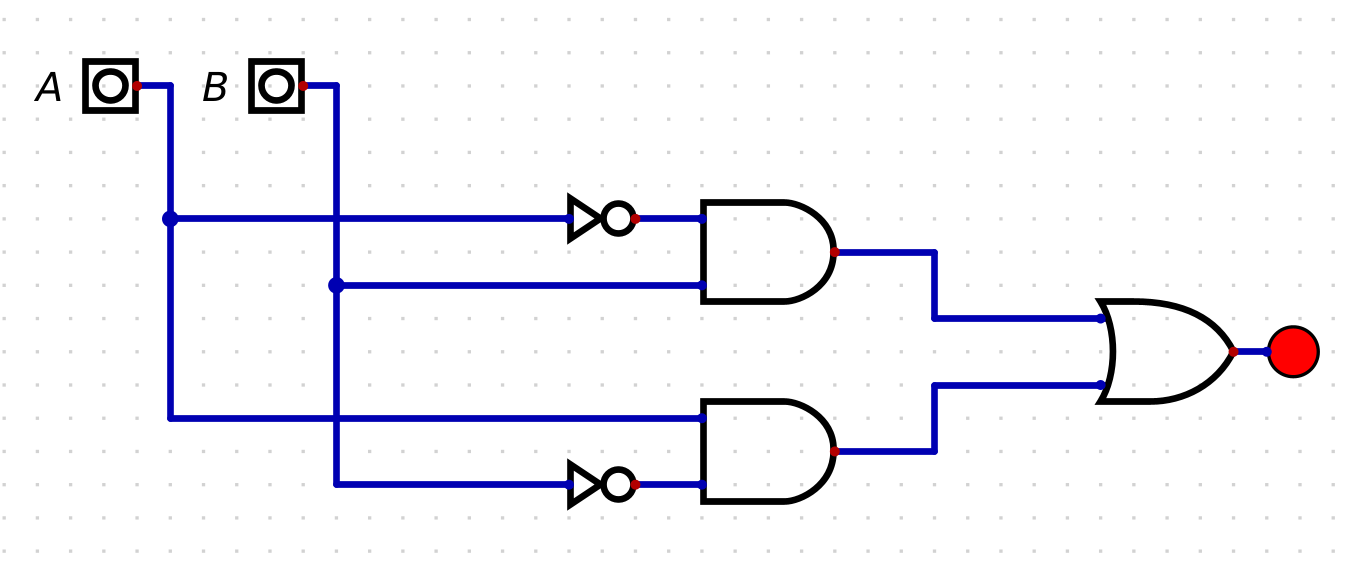
\includegraphics[width=0.5\textwidth]{img/cuircuito-xor.png}
	\end{figure}

	Reapre que o operador (E) na expressão é implícito enquanto no circuito
	sua construção é explícita. A expressão poderia também ser representada 
	da seguinte forma: $(\lnot{a} \land b) \lor (a \land \lnot{b})$, ou seja,
	são apenas formas diferentes de representar a mesma expressão, e, para
	melhorar a leitura, corriqueiramente podem ter representações implícitas
	nas expressões. \\
	\newline
	Observe agora a expressão: 
	$ ((a \oplus b \oplus c) \land \lnot{(b \lor d)}) \lor 
	\lnot{(\lnot{a} \land b \land c \lnot{d})} $ \\
	\newline
	Pode ser expressa físicamente pelo seguinte circuito:
	\begin{figure}[h]
		\centering
		\caption{circuitos/combinacionais/circuito-F.dig}
		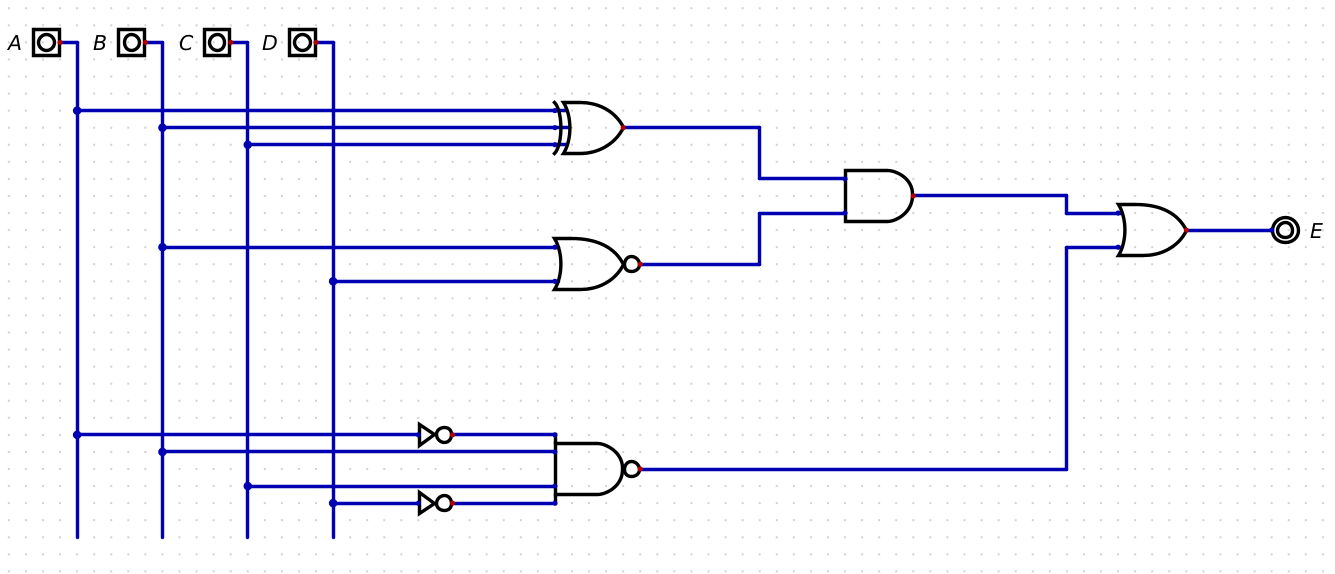
\includegraphics[width=0.5\textwidth]{img/circuito-F.png}
	\end{figure}
	
	Para finalizar e consolidar os conhecimentos em circuitos combinacionais
	vamos considerar o seguinte circuito:
	\begin{figure}[h]
		\centering
		\caption{circuitos/combinacionais/somador-completo.dig}
		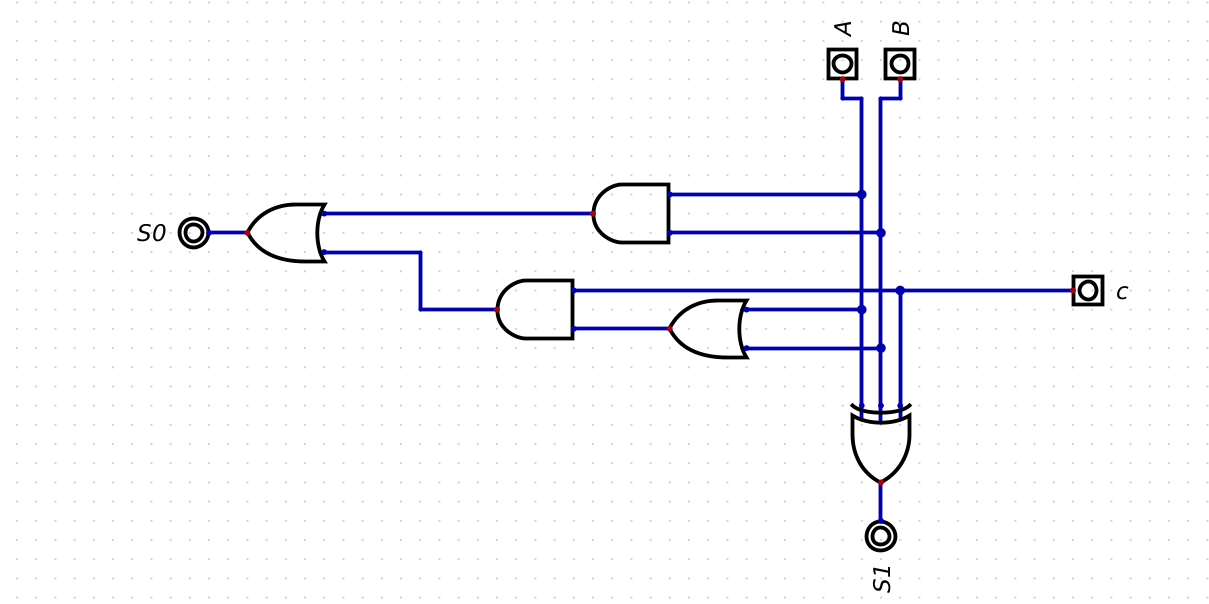
\includegraphics[width=0.5\textwidth]{img/somador.png}
	\end{figure}
	Repare que neste caso especifico temos duas saidas: S0 e S1
	e as entradas a, b, c.
	\newline
	Podemos obter as expressões a partir do curcuito acima, observe que
	para a saida S0 temos: $a \land e \lor (a \land b) \land c$ enquanto
	para saida S1 temos: $a \oplus b \oplus c$. 
	\newline
	Podemos perceber então a relação direta entre a construção de circuitos
	combinacionais utilizando blocos, ou seja, portas lógicas e também 
	a relação entre as expressões algébricas obtidas por uma análise 
	do circuito.

	\subsection{\centering Blocos Combinacionais Básicos}





	\bibliographystyle{apalike}
        \bibliography{ref.bib}

\end{document}
